\documentclass[a5paper,11pt,dvipdfmx]{tarticle}

\usepackage{okumacro}
\usepackage{graphicx}
\usepackage{wrapfig}

\renewcommand{\thesubsection}{\rensuji{\arabic{subsection}}}

\setlength{\columnsep}{2zw}
\setlength\intextsep{18pt}
\setlength\textfloatsep{18pt}
\usepackage[Q=10,W=46,L=18,ptj,tate]{hanmen}

\title{明解・四柱推命学(基礎編)}
\author{藤田 肇}

\begin{document}

%\tableofcontents
%\newpage

\section{四柱推命学の概要}
\subsection{四柱推命学とは}

四柱推命学は、人間が生まれた年・月・日・時に基づいて、その先天運命(持って生まれた質)と後天運勢(一生にわたる運気の流れ)とを推測する学問です。中国思想の陰陽五行説に端を発し、日本には文政年間(1818年頃)に中国から渡来したと考えられています。

中国では、古来より数々の思想家たちが、天体の運行、暦の記録、方角の指示、時間の測定などの複雑な事象を陰陽五行に則って体系化してきました。そして、四柱推命学は、その膨大な成果の積み上げに基づく「学問」として、長い歴史に耐えて現代まで発展を遂げてきました。成果と歴史の裏付けがあるからこそ、近代的な西洋の学問と同じように奥深く、東洋の学問の一つとして尊重されるべきものと言えます。

四柱推命学はあくまで学問であるため、霊感などの神がかり的な素養を必要としません。理屈を覚えて所定の手順に習熟すれば、誰でも先天運命と後天運勢を推測できます。つまり、推測の方法論がすべて言語化されているのです。もちろん、その手順は単純ではなく、習熟には時間を要しますし、推測の巧拙に応じてその精度は変わります。しかし、言語化により「誰でもできる」ことは1つの大きなポイントと言えるでしょう。

運命・運勢は、\ruby{命式}{めいしき}・\ruby{大運}{だいうん}を求めた上で、それらを解釈することによって推測できます。ここで、命式は、生年・月・日・時を列とした一種の表のように記述され、大運は、運勢を示す\ruby{干支}{かんし}を書き添えた一種の数直線のように記述されます。例えば、平成元年\rensuji{11}月\rensuji{26}日\rensuji{13}時\rensuji{45}分生まれの男性からは、次の命式(上部)と大運(下部)が求められます。

\begin{wrapfigure}{l}[0pt]{0.46\textwidth}
  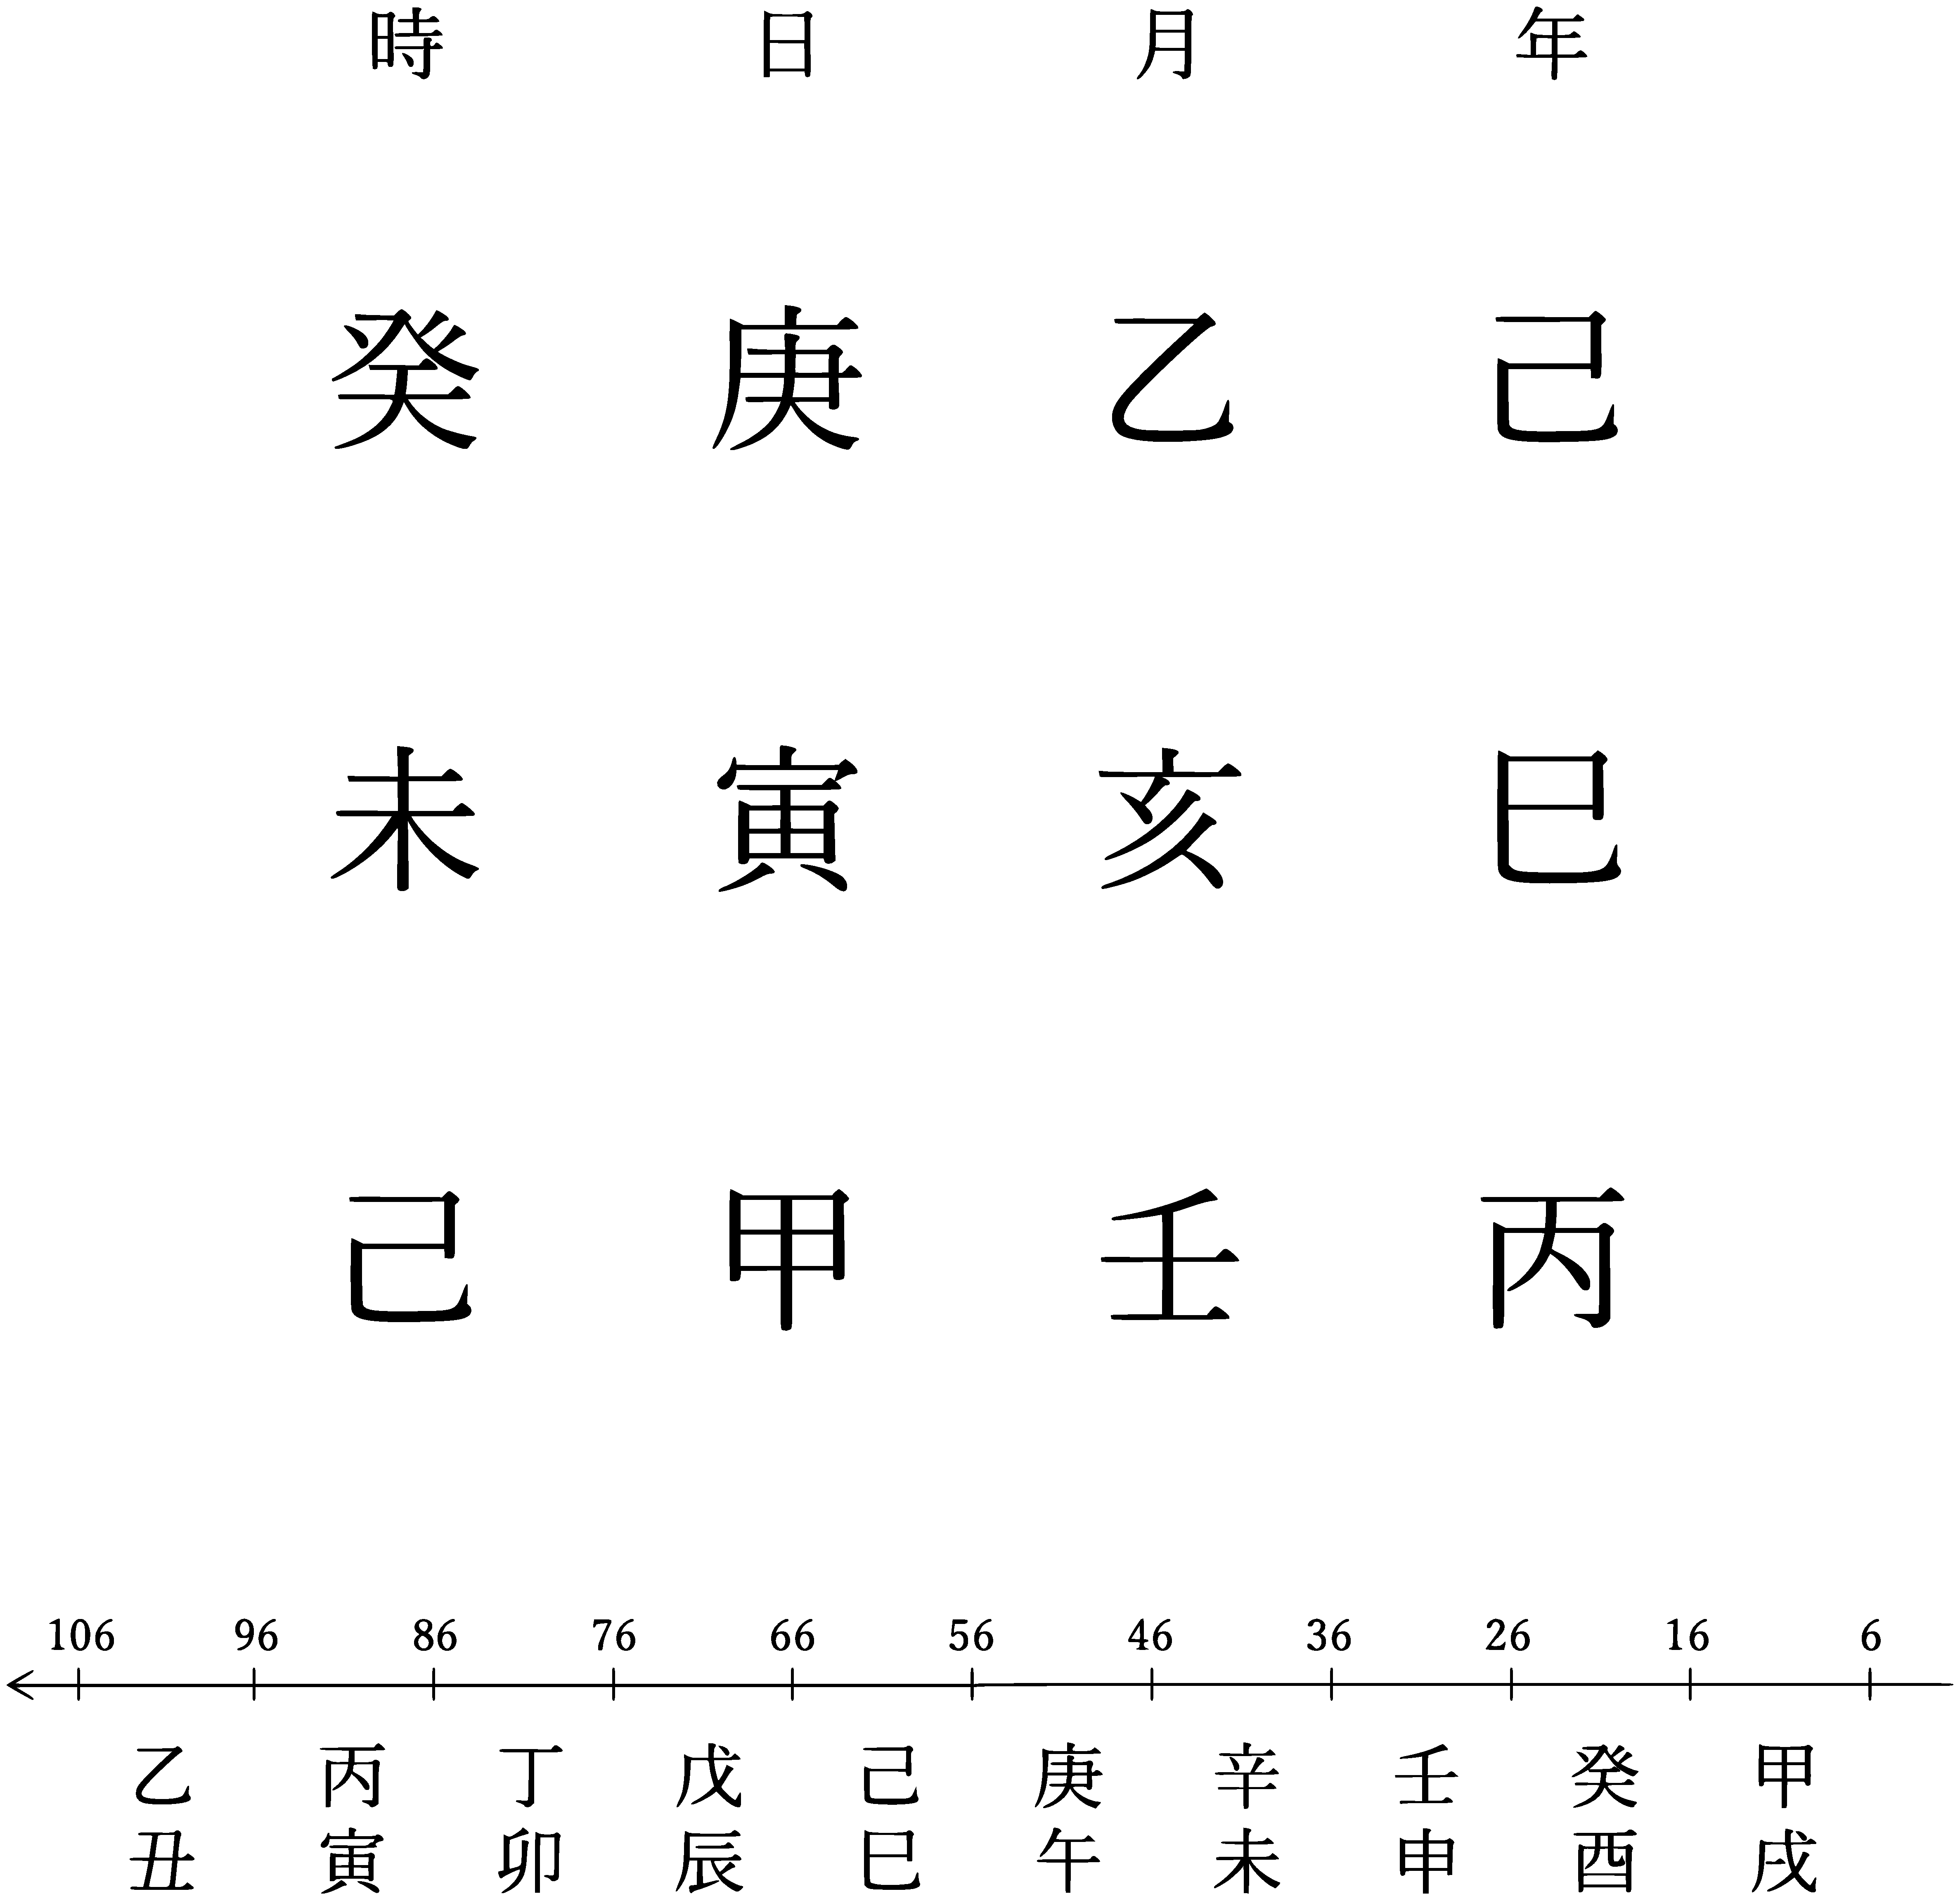
\includegraphics[width=79mm,angle=90]{figs/fig1.eps}
\end{wrapfigure}

命式は干支で表され、これがその人の持って生まれた先天運命を表します。命式を求める方法は機械的です。四柱推命学を志す人は、まずこれを求める方法に習熟する必要があります。

大運にもさまざまな要素が含まれ、これがその人の後天運勢を表します。命式と同様に、大運を求める方法も機械的です。やはりこれを求める方法にも習熟する必要があります。

命式・大運を求めた後、これらを詳細に解釈することによって、その人の運命・運勢を推測します。これにより、その人の性質、適職指向、人事・事相、肉親関係など、多岐にわたる事柄を明らかにできます。

例えば、先の男性は、才智に富み活動家と命式から推測できます。また、社交的で人間関係も良好ですが、積極性に欠けるところに注意が必要となるでしょう。さらに、\rensuji{45}歳までは良い運気が続きますが、それ以降は注意が必要となるため、若い時にできるだけ努力して将来に備えるべきことが、大運から推測できます。

このように、四柱推命学は、人間が生まれた年・月・日・時に基づいて、その先天運命と後天運勢とを推測する方法論です。各自の生まれながらに持っている質を知り、運気の流れを知り、人生航路で起きるさまざまな出来事や受難に対処する方法を考えるものです。

命式は、生年・月・日・時から一意に求められ、これは「持って生まれた運命」として換えようがありませんが、各人の人生が生まれながらに決定されているわけでは当然ありません。先天の運命が大輪の種子であったとしても、努力の時期を逸すれば花は咲きませんし、小さな草花の種子であったとしても、条件が整えば立派な花を咲かすことができます。四柱推命によって自分をよく知り、生涯の大局を見据えて、各自に応じた努力を積み重ねることにより、その後の運勢は必ず開かれるでしょう。


\subsection{五術体系における位置付け}

中国には、古来より「五術体系」と呼ばれる分類があります。\ruby{命}{めい}・\ruby{卜}{ぼく}・\ruby{相}{そう}・\ruby{医}{い}・\ruby{山}{ざん}の分類があり、これらはそれぞれ次の意味を持ちます。
\begin{description}
\item[\ruby{命}{めい}]命術のことで、生年・月・日・時に基づいて、先天運命と後天運勢とを推測する方法を指します。四柱推命はこの「命」に分類されます。その他、\ruby{紫微斗数}{しびとすう}、\ruby{九星気学}{きゅうせいきがく}などがこれにあたります。
\item[\ruby{卜}{ぼく}]卜術(\ruby{占卜}{せんぼく})のことで、偶然にあらわれた象徴を用いて、事柄や事態の成り行きを占う方法を指します。\ruby{周易}{しゅうえき}・\ruby{断易}{だんえき}・\ruby{梅花心易}{ばいかしんえき}などがこれにあたります。タロット・ルーンなども占卜に該当するでしょう。
\item[\ruby{相}{そう}]相術のことで、対象の姿・形から、その対象の状態や運勢を占う方法を指します。主なものとして、手相・人相・姓名判断・風水などがこれにあたります。
\item[\ruby{医}{い}]中国医術のことで、鍼灸・漢方・整体術などがこれにあたります。
\item[\ruby{山}{ざん}]大地自然の気をもらうことによって習得する術の総称で、気功・呼吸法・食事療法などがこれにあたります。
\end{description}

巷ではよく混同されていますが、四柱推命学は「占卜(占い)」ではありません。前述したとおり、「理屈」を積み上げて運命・運勢を推測する「命」であって、占卜のように「偶然」に頼る「卜」とは異なります。\footnote{そのため、サイコロやカードなどの小道具は一切用いません。}

そのため、「この時期にはこんなことが起こる」「この日は注意しなければ悪いことが起こる」「この時期に亡くなる」など、将来に起きる出来事を予言できるわけではありません。四柱推命学は、\ruby{看命}{かんめい}できる範囲は明確に決まっており、これを逸脱して不確かな推測を振り回すことを嫌います。\footnote{四柱推命学は「占い」ではないことから、対象を\ruby{看}{み}ることを「占う」とは言いません。「看命する」「鑑定する」などと言います。}

四柱推命学を真に志すのであれば、占卜との違いを理解した上で、理論・理屈から外れたことを云々することは控える自戒が必要です。

\subsection{概要のまとめ}
四柱推命学は「人間を知る学問」です。生年・月・日・時だけから、「命式」という航海図を描き、「大運」という天気予報を得る\ruby{命学}{めいがく}です。

こんな格言があります。\\

人事を尽くして天命を待つは常人なり

天命を知って人事を尽くすは達人なり\\

四柱推命学によって、各人が生まれながらに持っている天命(質)をよく知り、自分の生涯のうち、いつ花が咲くか、いつ注意すればよいかを予測します。そして、発展運の時は大いに伸ばし、凶運の時は大難を小難に止める人事を尽くせば、人生の「達人」といえるかもしれません。

それでは、奥深い四柱推命学の世界に足を踏み入れましょう。本書がその正しい第一歩となることを願っています。

\clearpage

\section{予備知識}

この章では、四柱推命学を学び進めるために必要となる最も基本的なことを解説します。普段は馴染みのない用語が多数出てきますが、少しずつ慣れていきましょう。

\subsection{陰陽五行と干支}
\subsubsection*{陰陽五行説}
陰陽説は、世界が陰と陽のバランスから成り立っていると考える思想です。例えば、「太陽と月」「天と地」「昼と夜」「男と女」「裏と表」など、自然界の全てのものを「陰」と「陽」の相反する二つの要素でとらえます。そして、これらが互いに消長し、調和することによって自然界の秩序が保たれていると解釈します。

一方で、五行説は、万物が\ruby{木}{もく}・\ruby{火}{か}・\ruby{土}{ど}・\ruby{金}{ごん}・\ruby{水}{すい}の五つの要素(五行)から構成されていると考える思想です。そして、これらの要素の盛衰・消長によって、この世のすべてが循環して進展すると解釈します。

そして「陰陽五行説」は、陰陽説と五行説とが結びついた古代中国の思想です。四柱推命学では、この陰陽五行説に基づいて、\textbf{陰陽・五行の均衡・不均衡を検討すること}が、最大のポイントとなります。

\subsubsection*{\ruby{十干}{じっかん}}

\begin{wrapfigure}{l}[0pt]{0.25\textwidth}
  
\includegraphics[width=85mm,angle=90]{figs/table2-1.eps}
\end{wrapfigure}

陰陽説によれば、すべてのものに陰陽がありますので、\ruby{木}{もく}・\ruby{火}{か}・\ruby{土}{ど}・\ruby{金}{ごん}・\ruby{水}{すい}の五行にもそれぞれ陰陽があることになります。

ここで、中国の慣習にしたがって陽を「\ruby{兄}{え}」に、陰を「\ruby{弟}{と}」に対応づけ、これらの陰陽五行の十種類を漢字で表現すると、上の表のようになります。

例えば、「\ruby{木}{もく}」の五行の陽は「\ruby{木}{き}の\ruby{兄}{え}」となり、「\ruby{甲}{きのえ}」の漢字で表現します。また、「\ruby{金}{ごん}」の五行の陰は「\ruby{金}{か}の\ruby{弟}{と}」となり、「\ruby{辛}{かのと}」の漢字で表現します。\footnote{「金」が変則的な読み方(ごん、か)になることに注意しましょう。}

このように、陰陽五行の十種類を漢字で表現したものを「\ruby{十干}{じっかん}」と呼びます。

また、\ruby{甲}{きのえ}・\ruby{丙}{ひのえ}・\ruby{戊}{つちのえ}・\ruby{庚}{かのえ}・\ruby{壬}{みずのえ}(\ruby{兄}{え}のグループ)を「\ruby{陽干}{ようかん}」と呼び、\ruby{乙}{きのと}・\ruby{丁}{ひのと}・\ruby{己}{つちのと}・\ruby{辛}{かのと}・\ruby{癸}{みずのと}(\ruby{弟}{と}のグループ)を「\ruby{陰干}{いんかん}」と呼びます。

四柱推命学では、この十干が一つの基礎になりますので、まずは漢字の表記と読みを正しく覚えておく必要があります。

\clearpage

\subsubsection*{\ruby{十二支}{じゅうにし}}

\begin{wrapfigure}{l}[0pt]{0.18\textwidth}
  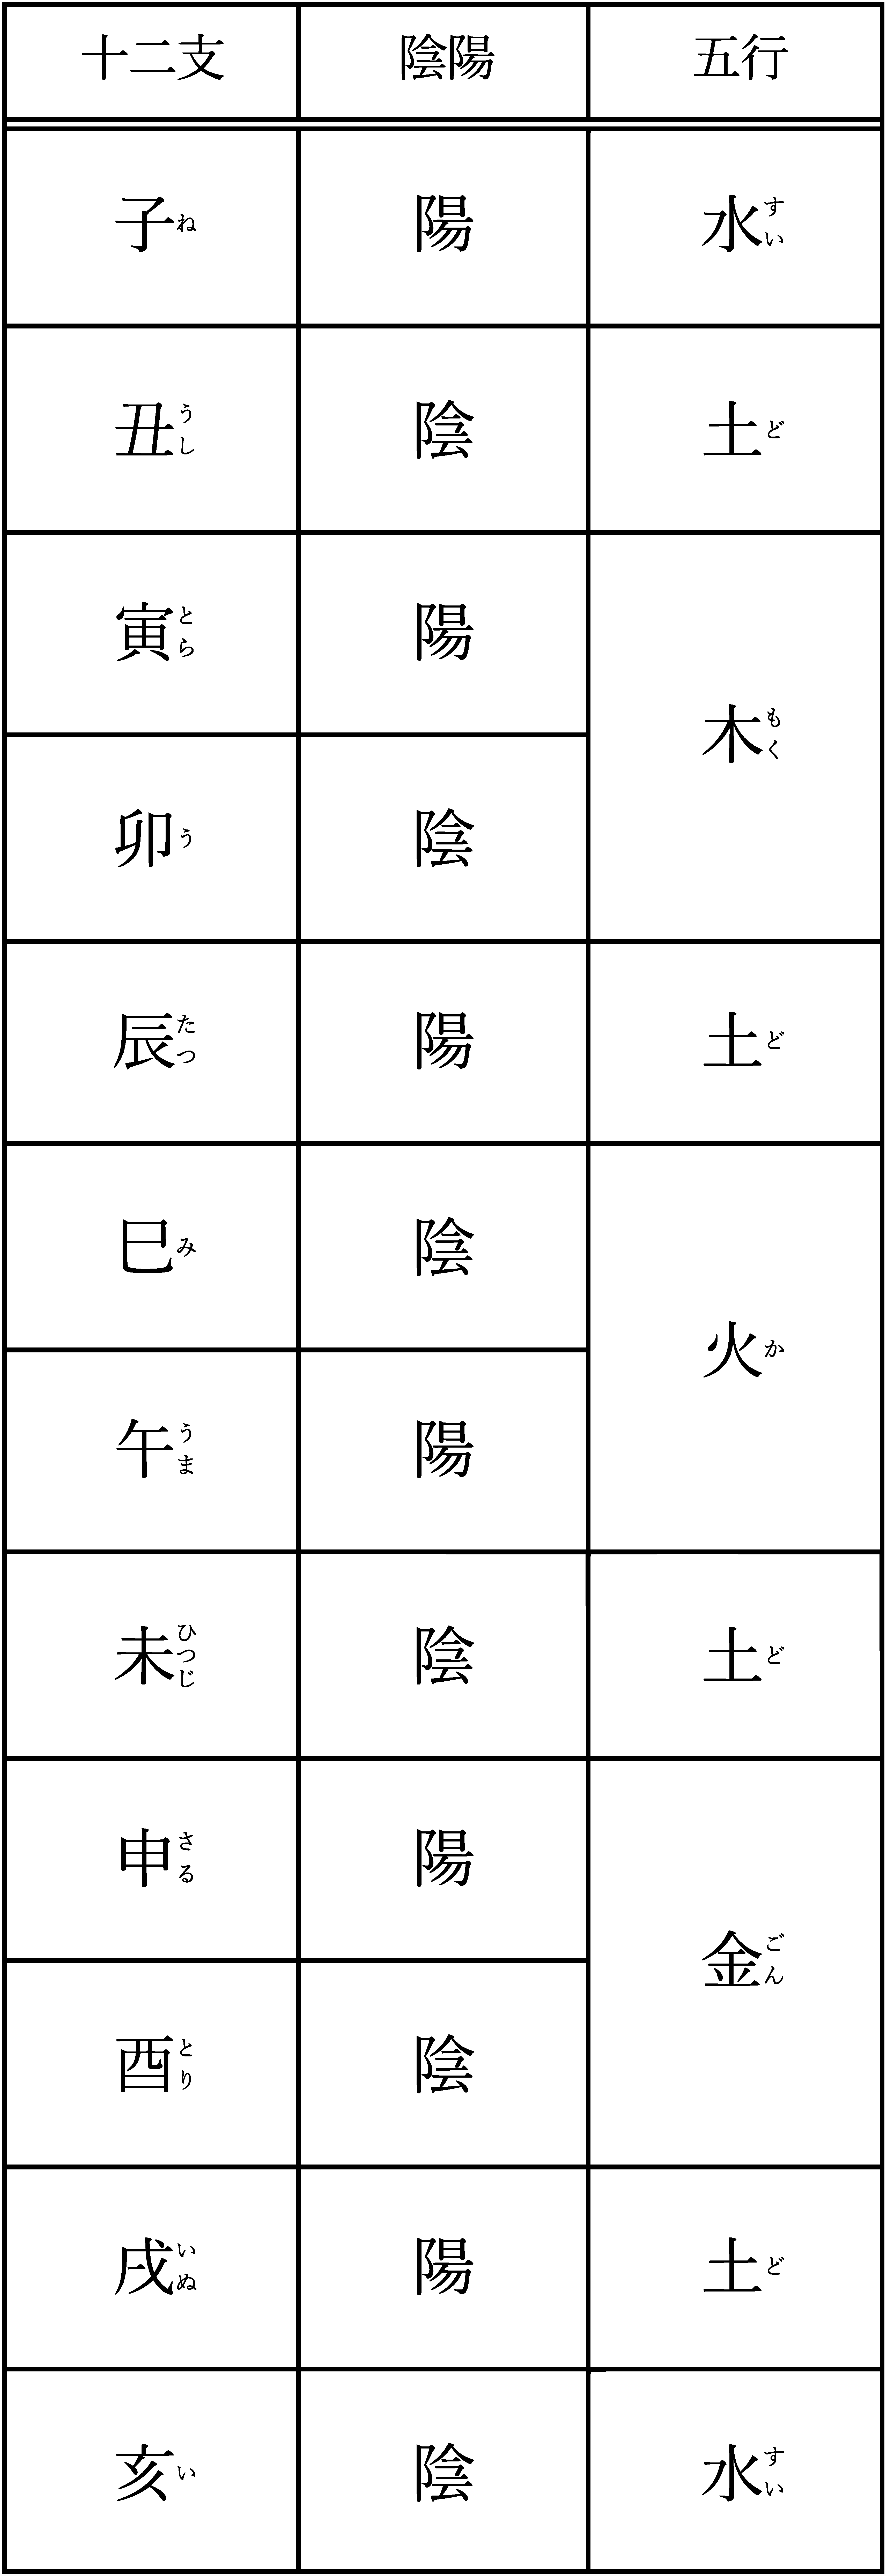
\includegraphics[width=85mm,angle=90]{figs/table2-2.eps}
\end{wrapfigure}

\ruby{十二支}{じゅうにし}は、\ruby{子}{ね}、\ruby{丑}{うし}、\ruby{寅}{とら}、\ruby{卯}{う}、\ruby{辰}{たつ}、\ruby{巳}{み}、\ruby{午}{うま}、\ruby{未}{ひつじ}、\ruby{申}{さる}、\ruby{酉}{とり}、\ruby{戌}{いぬ}、\ruby{亥}{い}の総称です。日本では年を表す\ruby{干支}{えと}として馴染み深いものです。

十二支にも陰陽・五行の分類があり、それぞれ上の表のようになります。

また、\ruby{子}{ね}・\ruby{寅}{とら}・\ruby{辰}{たつ}・\ruby{午}{うま}・\ruby{申}{さる}・\ruby{戌}{いぬ}を「\ruby{陽支}{ようし}」と呼び、\ruby{丑}{うし}・\ruby{卯}{う}・\ruby{巳}{み}・\ruby{未}{ひつじ}・\ruby{酉}{とり}・\ruby{亥}{い}を「\ruby{陰支}{いんし}」と呼びます。

四柱推命学では、命式・大運をすべて\ruby{十干}{じっかん}と\ruby{十二支}{じゅうにし}で表しますので、\ruby{十干}{じっかん}だけでなく、\ruby{十二支}{じゅうにし}の表記と読みも覚えておく必要があります。


\subsubsection*{\ruby{干支}{かんし}}

\ruby{十干}{じっかん}と\ruby{十二支}{じゅうにし}を合わせた十干十二支を「\ruby{干支}{かんし}」と略して呼びます。\ruby{干支}{えと}と漢字が同じですが、意味も読み方も異なりますので注意しましょう。\footnote{以後「干支」はすべて「かんし」と読みます。}

陽干と陽支、陰干と陰支を任意に組み合わせると、六〇通りの干支を構成できます。これを表にしたものを「\ruby{六十干支}{ろくじっかんし}表」と呼びます。\footnote{表の最下段に記載の「空亡」については、後の章で詳しく説明します。}

\begin{figure}
  \centering
  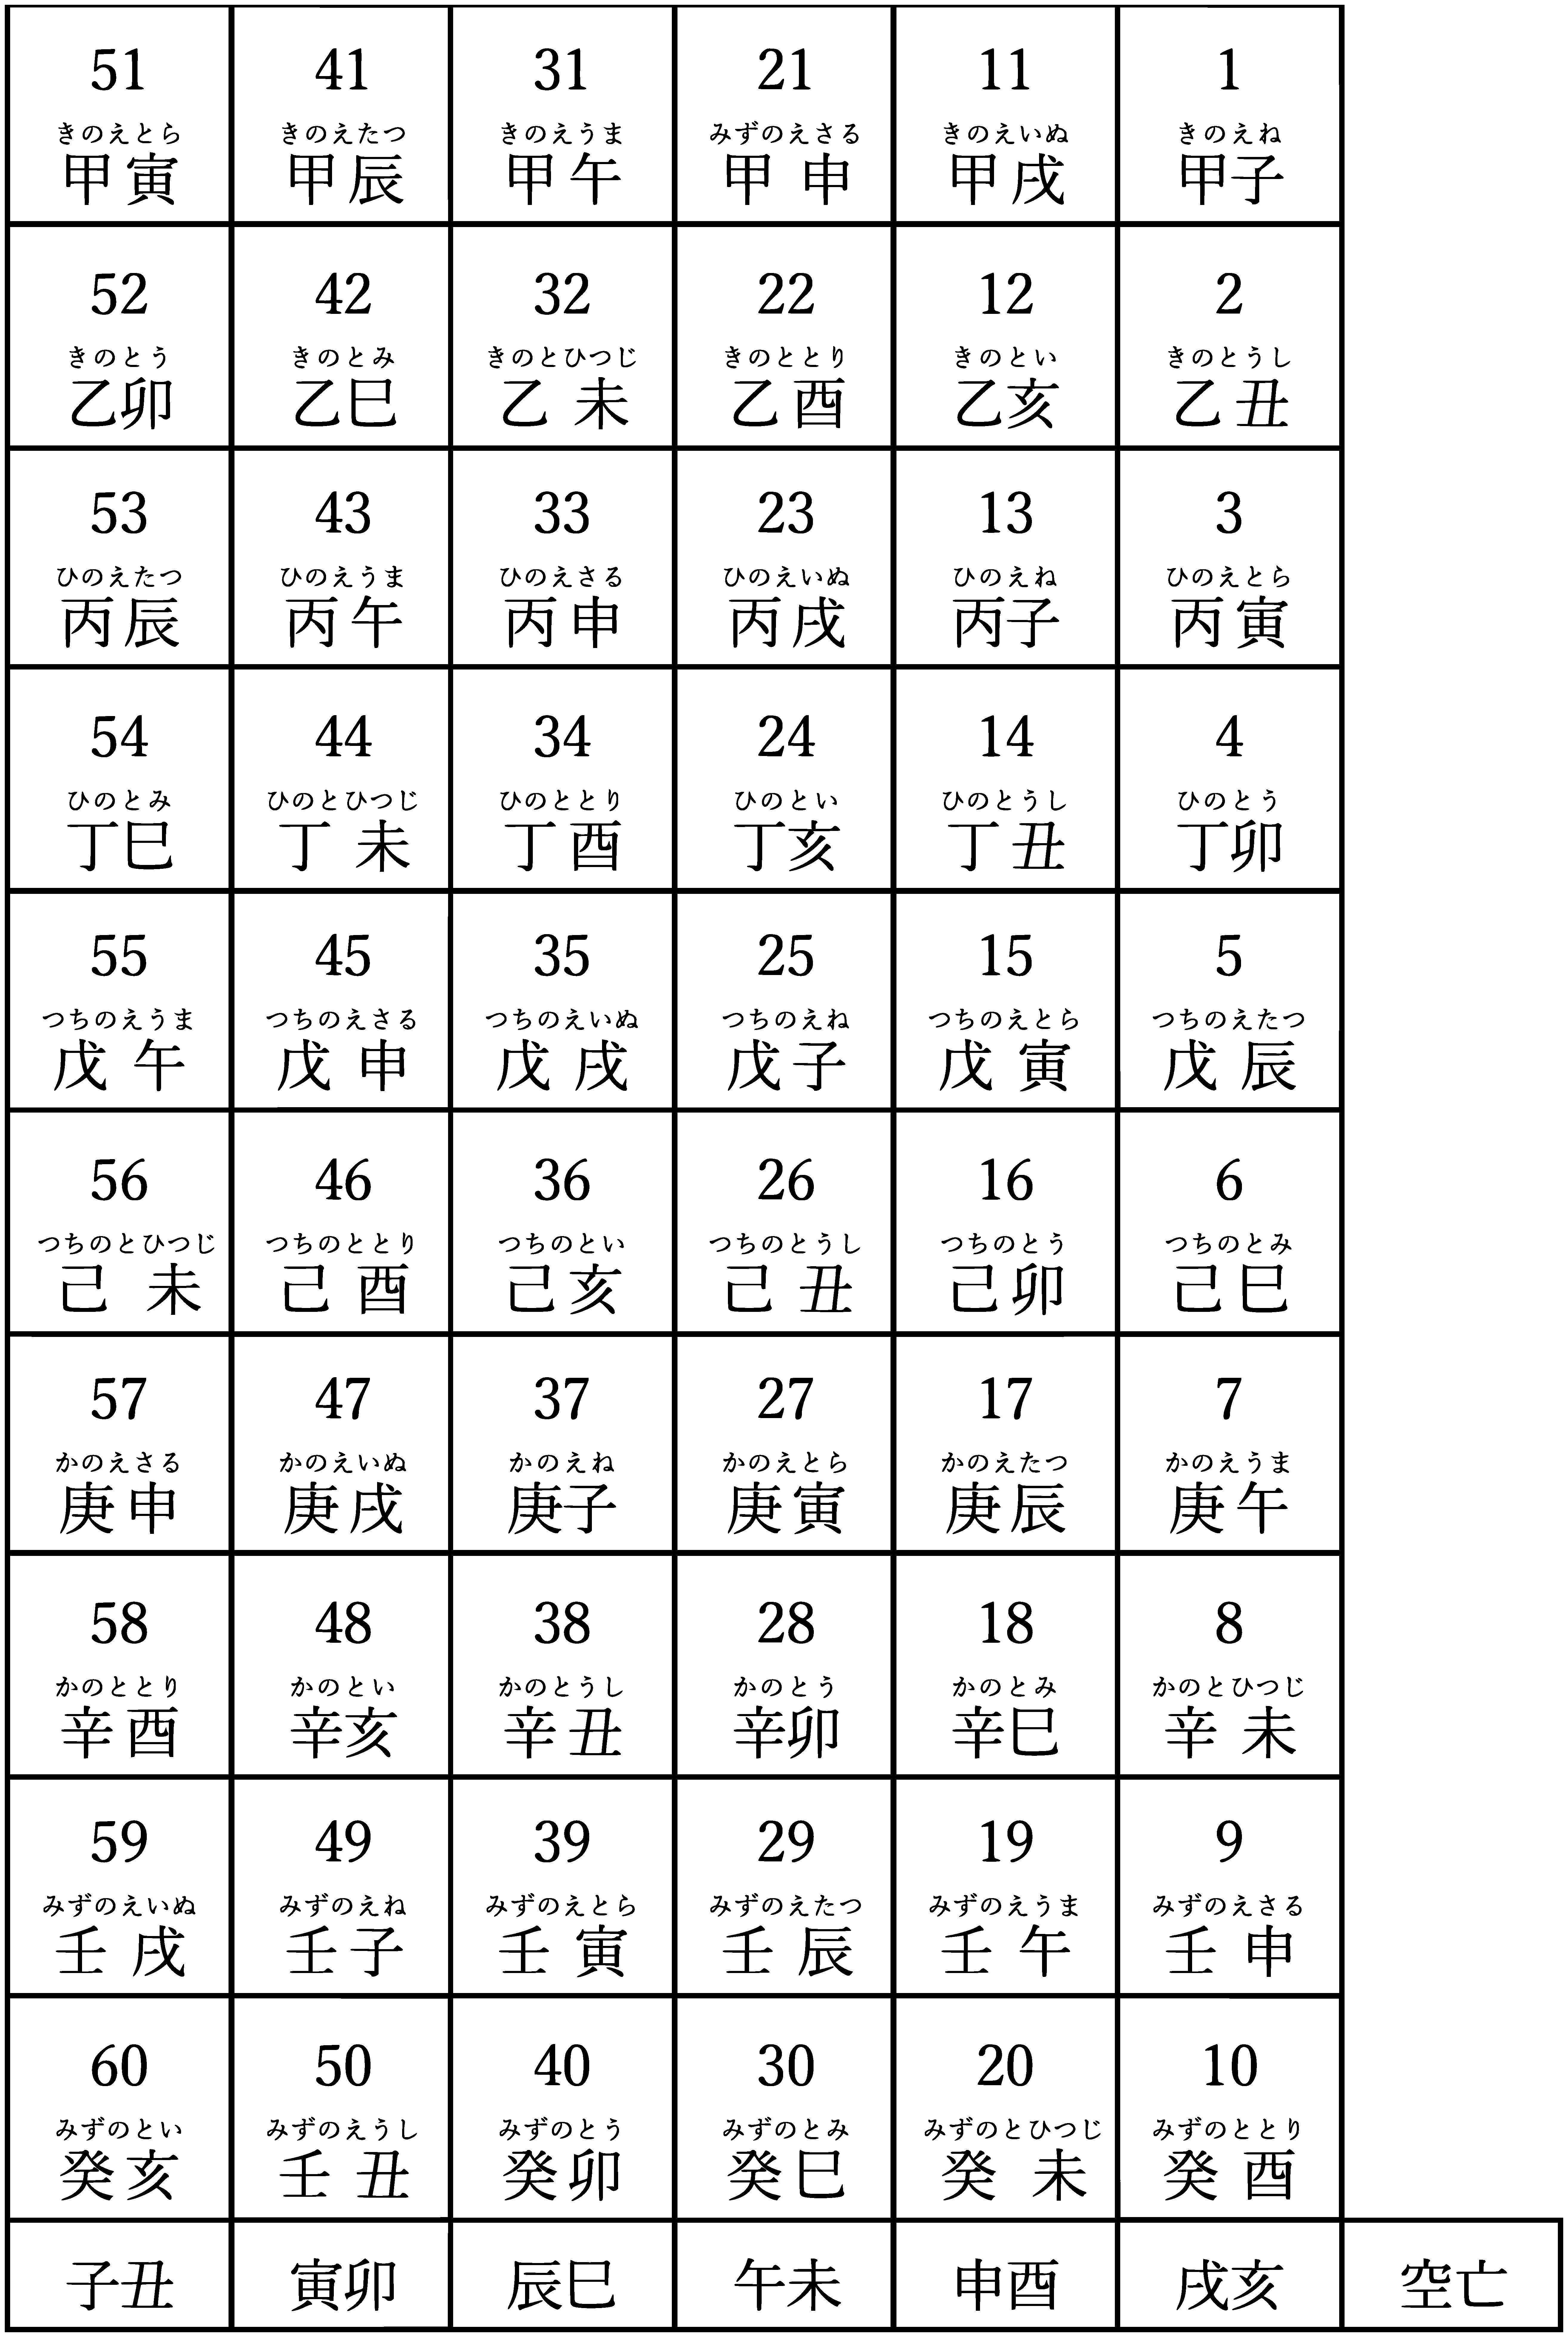
\includegraphics[width=95mm,angle=90]{figs/table2-3.eps}
\end{figure}

\clearpage

中国では、古代からこの六十干支を用いて暦を記録していました。私たちが普段使う近代西洋の「\ruby{天文暦}{てんもんれき}」に対して、これを「\ruby{干支暦}{かんしれき}」と呼びます。

六十干支は、表のように「\ruby{甲子}{きのえね}」(1)から始まり「\ruby{癸亥}{みずのとい}」(\rensuji{60})で終わります。一巡すると、また「\ruby{甲子}{きのえね}」から始まり、この六十干支表の番号順に、年・月・日・時の干支が延々と巡ります。

例えば、最近では大正\rensuji{13}年(1924年)が「\ruby{甲子}{きのえね}」であり、それより六〇年後の昭和\rensuji{59}年(1984年)も「\ruby{甲子}{きのえね}」でした。同様に、2044年も「\ruby{甲子}{きのえね}」になります。余談ですが、甲子園球場は、大正\rensuji{13}年の「\ruby{甲子}{きのえね}」年に完成したことにちなんで、その名が付けられました。六〇歳を「還暦」と呼ぶのも、「暦が\ruby{還}{かえ}る」ことからきています。

また、令和3年(2022年)8月は「\ruby{己酉}{つちのととり}」であり、同月\rensuji{17}日は「\ruby{壬寅}{みずのえとら}」でした。そのため、六〇月後の令和8年(2027年)8月も「\ruby{己酉}{つちのととり}」であり、六〇日後の\rensuji{10}月\rensuji{16}日も「\ruby{壬寅}{みずのえとら}」でした。

さらに、令和元年(2019年)5月\rensuji{13}日\rensuji{13}時0分は「\ruby{癸未}{みずのとひつじ}」だったため、六〇時間後の同月\rensuji{18}日\rensuji{13}時0分も「\ruby{癸未}{みずのとひつじ}」でした。

このように、年・月・日・時の干支が、古代から六〇サイクルにより休みなく巡っています。

四柱推命学では、\textbf{天文暦で表される生年・月・日・時を、干支暦で表される生年・月・日・時に置き換えることが最初の一歩}となります。


\subsection{五行と季節の関係}

\ruby{木}{もく}・\ruby{火}{か}・\ruby{土}{ど}・\ruby{金}{ごん}・\ruby{水}{すい}の五行には、次の表のようにそれぞれ季節が対応づけられています。

【表2ー4】

「木」が青葉となり茂る季節が春、「火」が燃えるように暑くなる季節が夏、「金」が土の中で実る季節が秋、「水」が冷たく凍る季節が冬に対応します。「土」は、それぞれの季節の終わりを表し、これを「土用」といいます。\footnote{いわゆる「土用の丑」は、暦の上での夏(七月)の土用(立秋まえの十八日間)をいいます。}

四柱推命学は季節を重視します。人間の運勢にも「季節」があり、その移ろいに応じて人生にさまざまな変化をもたらすと考えるからです。

例えば、大運に「春」が巡った場合、命式に含まれる木の五行(\ruby{甲}{きのえ}、\ruby{乙}{きのと})が\ruby{旺}{おう}じます。\footnote{「\ruby{旺}{おう}じる」とは、その五行の作用が大きくなることをいいます。}

同様に、「夏」が巡った場合は火の五行(\ruby{丙}{ひのえ}、\ruby{丁}{ひのと})が、「秋」が巡った場合は金の五行(\ruby{庚}{かのえ}、\ruby{辛}{かのと})が、「冬」が巡った場合は水の五行(\ruby{壬}{みずのえ}、\ruby{癸}{みずのと})が旺じます。そして、それぞれの季節の終わり(土用)には土の五行(\ruby{戊}{つちのえ}、\ruby{己}{つちのと})が旺じます。その結果、命式において他の五行との相対的な関係がダイナミックに変化し、これが運勢の吉凶を決定づけることになります。


\subsection{予備知識のまとめ}

四柱推命学の予備知識として、五行、十干、十二支、季節について説明しましたが、この内容をあらためて表にすると次のようになります。

【表2―5】

まとめると、まず五行(\ruby{木}{もく}・\ruby{火}{か}・\ruby{土}{ど}・\ruby{金}{ごん}・\ruby{水}{すい})があり、これらの陰陽によって\ruby{十干}{じっかん}(\ruby{甲}{きのえ}、\ruby{乙}{きのと}、\ruby{丙}{ひのえ}、\ruby{丁}{ひのと}、\ruby{戊}{つちのえ}、\ruby{己}{つちのと}、\ruby{庚}{かのえ}、\ruby{辛}{かのと}、\ruby{壬}{みずのえ}、\ruby{癸}{みずのと})が導かれます。そして、この十干と十二支(\ruby{子}{ね}、\ruby{丑}{うし}、\ruby{寅}{とら}、\ruby{卯}{う}、\ruby{辰}{たつ}、\ruby{巳}{み}、\ruby{午}{うま}、\ruby{未}{ひつじ}、\ruby{申}{さる}、\ruby{酉}{とり}、\ruby{戌}{いぬ}、\ruby{亥}{い})とを合わせて「\ruby{干支}{かんし}」と呼びます。人間の先天運命を表す命式も後天運勢を表す大運も、すべてこの干支で表現されます。

五行には季節が対応づけられています。\ruby{木}{もく}が春、\ruby{火}{か}が夏、\ruby{土}{ど}が土用、\ruby{金}{ごん}が秋、\ruby{水}{すい}が冬です。そして、十干では\ruby{甲}{きのえ}、\ruby{乙}{きのと}が、十二支では\ruby{寅}{とら}、\ruby{卯}{う}が「春」に対応します。同様に、\ruby{丙}{ひのえ}、\ruby{丁}{ひのと}、\ruby{巳}{み}、\ruby{午}{うま}が「夏」、\ruby{戊}{つちのえ}、\ruby{己}{つちのと}、\ruby{丑}{うし}、\ruby{辰}{たつ}、\ruby{未}{ひつじ}、\ruby{戌}{いぬ}が「土用」、\ruby{庚}{かのえ}、\ruby{辛}{かのと}、\ruby{申}{さる}、\ruby{酉}{とり}が「秋」、\ruby{壬}{みずのえ}、\ruby{癸}{みずのと}、\ruby{亥}{い}、\ruby{子}{ね}が「冬」に対応します。

このように、四柱推命学は陰陽五行説に立脚しており、これに基づいて陰陽・五行の均衡・不均衡を検討することがすべての基本となります。そのため、まずは五行・十干・十二支、およびこれらの季節との対応を、予備知識としてしっかり覚えておきましょう。


\clearpage

\section{命式}

\ruby{命式}{めいしき}は、生年・月・日・時を「\ruby{干支}{かんし}」に置き換え、「\ruby{年柱}{ねんちゅう}」「\ruby{月柱}{げっちゅう}」「\ruby{日柱}{にっちゅう}」「\ruby{時柱}{じちゅう}」として組み立てたものです。

男性の命式を「\ruby{男命}{だんめい}」、女性の命式を「\ruby{女命}{じょめい}」といい、主に先天運命を推測する(推命する)ために用います。このように、年・月・日・時に対応する干支を「四つの柱」として推命するため、「四柱推命」と称します。

命式において、上段の干を「\ruby{天干}{てんかん}」、中段の支を「\ruby{地支}{ちし}」、下段の干を「\ruby{蔵干}{ぞうかん}」と呼びます。特に重要な干支は、日柱に位置する天干と、月柱に位置する地支であり、これらをそれぞれ「\ruby{日干}{にっかん}」、「\ruby{月支}{げっし}」と略して呼びます。\footnote{月支ほど頻出ではありませんが、年柱地支を「年支」、日柱地支を「日支」、時柱地支を「時支」と呼ぶことがあります。また、日干のことを「\ruby{日元}{にちげん}」「\ruby{命主}{めいしゅ}」「\ruby{日主}{にっしゅ}」ということもあります。}

【図3ー1】

命式は、天文暦で表される生年・月・日・時を、干支暦で表される生年・月・日・時に置き換えることで四柱干支を求め、次に蔵干を導くという手順で構成するため、ここではこの順序で説明します。

\subsection{四柱干支の求め方}
\subsubsection*{年の干支の求め方}

和暦から年干支を得る手順は、次のとおりです。

\begin{enumerate}
\item 昭和であれば2を足し、平成であれば5を足し、令和であれば\rensuji{35}を足す(足した数が\rensuji{60}を超過している場合は\rensuji{60}を引く)
\item 足した数に対応する干支を六十干支表から得る
\end{enumerate}

例えば、平成\rensuji{10}年の場合、\rensuji{10}に5を足すと\rensuji{15}です。そこで、六十干支表の\rensuji{15}に対応する干支「戊寅」を得ます。

昭和\rensuji{59}年の場合、2を足すと\rensuji{61}となり、\rensuji{60}を超えてしまいます。この場合はさらに\rensuji{60}を引いて1とし、六十干支表の1に対応する干支「甲子」を得ます。

なお、西暦から年干支を求める手順は、次のとおりです。
\begin{enumerate}
\item 3を引く
\item 残りの数から直近の\rensuji{60}の倍数を引く
\item 引いた数に対応する干支を六十干支表から得る
\end{enumerate}

例えば、1998年の場合、まず3を引くと1995となり、ここから1980(直近の\rensuji{60}の倍数)を引くと\rensuji{15}です。そこで、六十干支表の\rensuji{15}に対応する干支「戊寅」を得ます。

年柱の干支を求める場合、注意しなければならないことがあります。それは、立春前までに誕生した人については、前年の干支を採用するということです。立春とは、暦の上で春に入る日であり、節分の翌日のことです。なお、暦の上での各月の始まりに入ることを「\ruby{節入}{せつい}りする」といいます。

この注意事項を、次の図を用いて説明します。

【図3ー2】

一般に、平成\rensuji{10}年は、その年の1月1日から\rensuji{12}月\rensuji{31}日までのことです。

一方で、四柱推命学では、平成\rensuji{10}年として「戊寅」の年柱を採用するのは、平成\rensuji{10}年2月4日9時\rensuji{57}分の節入りから、平成\rensuji{11}年2月4日\rensuji{15}時\rensuji{57}分の節入りより前までです。\footnote{立春の日付と正確な時刻については、国立天文台が発行する「理科年表」で毎年発表されています。}

例えば、平成\rensuji{10}年1月は、まだ「戊寅」には節入りしていませんので、その前年の「丁丑」を採用します。同様に、平成\rensuji{11}年2月1日も、まだ「己卯」に節入りしていませんので、その前年の「戊寅」を採用します。

このように、1月から2月の立春より前に生まれた人の年柱の求め方は変則的になるので、注意が必要です。


\subsubsection*{月の干支の求め方}

月の干支は、次の月干支表を用いて求めます。

【表3ー1】

平成\rensuji{10}年\rensuji{11}月を例として説明します。

前述のとおり、年の干は「戊」でしたので、月干支表の「戊」の行を参照します。この表によれば、「戊」の「\rensuji{11}月亥」は「癸」です。そのため、平成\rensuji{10}年\rensuji{11}月の月干支は「癸亥」になります。

次に、昭和\rensuji{61}年9月を例として説明します。

六十干支表によれば、\rensuji{61}+2−\rensuji{60}=3の干支は「丙寅」ですので、これが年干支になります。月干支表の「丙」の行において「9月酉」は「丁」です。そのため、昭和\rensuji{61}年9月の月干支は「丁酉」になります。

最後に、平成8年1月を例として説明します。

六十干支表によれば、8+5=\rensuji{13}の干支は「丙子」です。しかし、1月はまだ節入りしていないので、年干支はその前年の「乙亥」になります。月干支表の「乙」の行において「1月丑」は「己」です。そのため、平成8年1月の月干支は「己丑」になります。

月干支を求める場合も、毎月の節入りを考慮する必要があることに注意が必要です。つまり、毎月の節入り前までに誕生した人については、前月の干支を採用するということです。\footnote{毎月の節入りは、\ruby{小寒}{しょうかん}(1月6日頃)、\ruby{立春}{りっしゅん}(2月4日頃)、\ruby{啓蟄}{けいちつ}(3月6日頃)、\ruby{清明}{せいめい}(4月5日頃)、\ruby{立夏}{りっか}(5月6日頃)、\ruby{芒種}{ぼうしゅ}(6月6日頃)、\ruby{小暑}{しょうしょ}(7月7日頃)、\ruby{立秋}{りっしゅう}(8月8日頃)、\ruby{白露}{はくろ}(9月8日頃)、\ruby{寒露}{かんろ}(\rensuji{10}月9日頃)、\ruby{立冬}{りっとう}(\rensuji{11}月8日頃)、\ruby{大雪}{だいせつ}(\rensuji{12}月7日頃)です。それぞれの日付と正確な時刻については、「理科年表」で発表されています。}

この注意事項を、次の図を用いて説明します。

【図3ー3】

一般に、平成\rensuji{10}年\rensuji{11}月は、\rensuji{11}月1日から\rensuji{11}月\rensuji{30}日までのことです。

一方で、四柱推命学では、平成\rensuji{10}年\rensuji{11}月「癸亥」の月柱を採用するのは、平成\rensuji{10}年\rensuji{11}月8日0時8分の節入り(立冬)から、同年\rensuji{12}月7日\rensuji{17}時2分の節入り(大雪)より前までです。

例えば、平成\rensuji{10}年\rensuji{11}月5日は、まだ「癸亥」には節入りしていませんので、その前月の「壬戌」を採用します。同様に、同年\rensuji{12}月2日は、まだ「甲子」に節入りしていませんので、「癸亥」を採用します。

このように、各月の上旬に生まれた人の月柱の求め方は変則的になるので、注意が必要です。

なお、月干支表の○内数字は「標準節入日」です。例えば、毎年8月の節入り(立秋)は、正確な時刻は別として「だいたい8日」です。そのため、「8月申」の下に「\textcircled{\rensuji{8}}」と記載しています。

この標準節入日を参考にして、節入りの有無を大まかに検討し、当月の干支を採用するか、前月の干支を採用するかを判断すればよいでしょう。


\subsubsection*{日の干支の求め方}

日干支は、次の生日基数表を用いて求めます。

【表3ー2】

日干支を求める手順は、次のとおりです。

\begin{enumerate}
\item 生日基数表から年月に対応する基数を得る
\item その基数に日の数を足す(足した数が\rensuji{60}を超過している場合は\rensuji{60}を引く)
\item 足した数に対応する干支を六十干支表から得る
\end{enumerate}

平成\rensuji{10}年\rensuji{11}月\rensuji{10}日を例として説明します。

生日基数表によれば、平成\rensuji{10}年\rensuji{11}月に対応する基数は「\rensuji{48}」です。これに日の数(\rensuji{10})を足すと「\rensuji{58}」です。六十干支表において「\rensuji{58}」に対応する干支は「辛酉」ですので、平成\rensuji{10}年\rensuji{11}月\rensuji{10}日の干支は「辛酉」になります。

次に、昭和\rensuji{61}年9月\rensuji{27}日を例として説明します。

生日基数表によれば、昭和\rensuji{61}年9月に対応する基数は「\rensuji{44}」です。これに日の数(\rensuji{27})を足すと「\rensuji{71}」です。\rensuji{60}を超えているので、\rensuji{71}から\rensuji{60}を引いて\rensuji{11}を得ます。六十干支表において「\rensuji{11}」に対応する干支は「甲戌」ですので、昭和\rensuji{61}年9月\rensuji{27}日の干支は「甲戌」になります。


\subsubsection*{時の干支の求め方}

時の干支は、次の時干支表を用いて求めます。

【表3ー3】

平成\rensuji{10}年\rensuji{11}月\rensuji{10}日\rensuji{13}時\rensuji{45}分を例として説明します。

前述のとおり、日干は「辛」でしたので、時干支表の「辛」の行を参照します。この表によれば、「辛」の「\rensuji{13}時より未」は「乙」です。そのため、平成\rensuji{10}年\rensuji{11}月\rensuji{10}日\rensuji{13}時\rensuji{45}分の時干支は「乙未」になります。

次に、昭和\rensuji{61}年9月\rensuji{27}日8時\rensuji{51}分を例として説明します。

前述のとおり、日干は「甲」でしたので、時干支表の「甲」の行を参照します。この表によれば、「甲」の「7時より辰」は「戊」です。そのため、昭和\rensuji{61}年9月\rensuji{27}日8時\rensuji{51}分の時干支は「戊辰」になります。



\end{document}
